\documentclass[handout]{beamer}

\usepackage{fontspec} 
% \usepackage{lsp-makros}
\useoutertheme{lsp}

\usepackage{lsptitle}

\def\two@digits#1{\ifnum#1<10 0\fi\number#1}
\def\mytoday{\two@digits{\number\day}.\two@digits{\number\month}.\number\year}


\usepackage{xspace,multicol}
\newcommand{\latex}{\LaTeX\xspace}
\usepackage{tikz}


\newcounter{lastpagemainpart}
\footnotesep0pt
\renewcommand{\footnoterule}{}
\usefootnotetemplate{
  \noindent
  \insertfootnotemark\insertfootnotetext}

\let\beamerfn=\footnote
\renewcommand{\footnote}[1]{%
\let\oldfnsize=\footnotesize%
\let\footnotesize=\tiny%
\beamerfn<\thebeamerpauses->{#1}%
\let\footnotesize=\oldfnsize}


\date{2018-06-23}

\usepackage{eurosym}  
 
\renewcommand{\centerline}[1]{\hfill#1\hfill\hfill\mbox{}}


\title{Full disclosure: Open Business Data and the Publisher's Cookbook}
\institute{ElPub 2018, Toronto}
\author[LangSci]{Sebastian Nordhoff \& Felix Kopecky}

% 15min

\begin{document}
\lspbeamertitle

% \section{some section}

\section{Metallurgy}
 
\frame{
\frametitle{OA metallurgy according to JS Caux}

\begin{columns}
  \begin{column}{7cm}
  \begin{itemize}
    \item \textbf{Gold [Au]} 	
    \begin{itemize}
     \item APC-based financing
    \end{itemize}
    \item \textbf{Platinum [Pt]} 	
    \begin{itemize}
     \item no charges for authors (APCs, submission charges or any other)
     \item funded through a consortial scheme or equivalent
    \end{itemize}
    \item \textbf{Palladium [Pd]} 
    \begin{itemize}
     \item purely not-for-profit public enterprise 
     \item none of the activities generate any profit
     \item all financial statements are publicly disclosed
    \end{itemize}
%     \bigskip
%     \pause 
%     \item Iron [Fe]	subscription-based financing, or pay-to-read
%     \item Lead [Pb] 	editorial and financial aspects are not hermetically decoupled
  \end{itemize}
  \end{column}
  \begin{column}{4cm}
    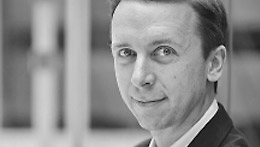
\includegraphics[width=4cm]{jscaux.jpg}\vfill	
\footnotesize
\url{https://jscaux.org/blog/post/2017/09/20/noble-metals-noble-cause/}
  \end{column}  
\end{columns}
} 

\frame{
\frametitle{OA metallurgy according to JS Caux}
% \begin{columns}
\begin{itemize}
 \item \textbf{10-karat} 	generosity to \textsc{readers}:
open access 	 
 \item \textbf{14-karat} 	generosity to \textsc{authors}:
no copyright transfer , no embargo 	
 \item \textbf{18-karat} 	generosity to \textsc{users}:
reuse, remix, crawl, citations 	
 \item \textbf{22-karat} 	generosity to \textsc{reviewers}:
open reports 	
 \item \textbf{24-karat} 	generosity to \textsc{community}:
academic control
\end{itemize}
}


\frame{
\frametitle{Language Science Press}
    \begin{itemize}
      \item 24kt Palladium OA publisher for books in linguistics
      \item DFG grant 2014-2016
      \item 20 series from phonetics to African linguistics to computational linguistics 
      \item 70 books published as of today
      \item today financed by 101 institutions worldwide (1000 EUR/yr) via Knowledge Unlatched
      \item \url{langsci-press.org}
    \end{itemize}
}

\frame{
\frametitle{Language Science Press}
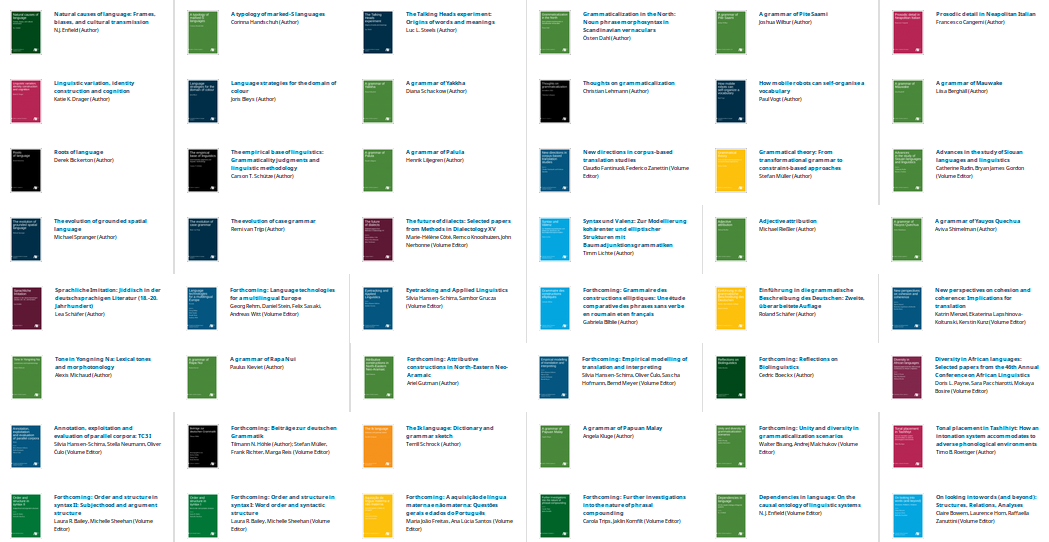
\includegraphics[width=\textwidth]{catalog.png}
}

\section{Full disclosure}
\frame{
\frametitle{Full Disclosure}
\fbox{ 
  \parbox{\textwidth}{
    \begin{itemize} 
    \item \textbf{Palladium [Pd]} 
      \begin{itemize}
      \item \dots
      \item all financial statements are publicly disclosed
      \end{itemize}
    \end{itemize}
  }
}
\begin{itemize}
\item OpenAire project ``Full disclosure: replicable strategies for book publications supplemented with empirical data''   
  \begin{enumerate}
  \item business data 
  \item spreadsheet
  \item business model 
  \item cookbook
  \end{enumerate}
\item \url{github.com/langsci/opendata}  
\end{itemize}
}

\section{Data}
\frame{
\frametitle{\mbox{Business data: Download figures}}
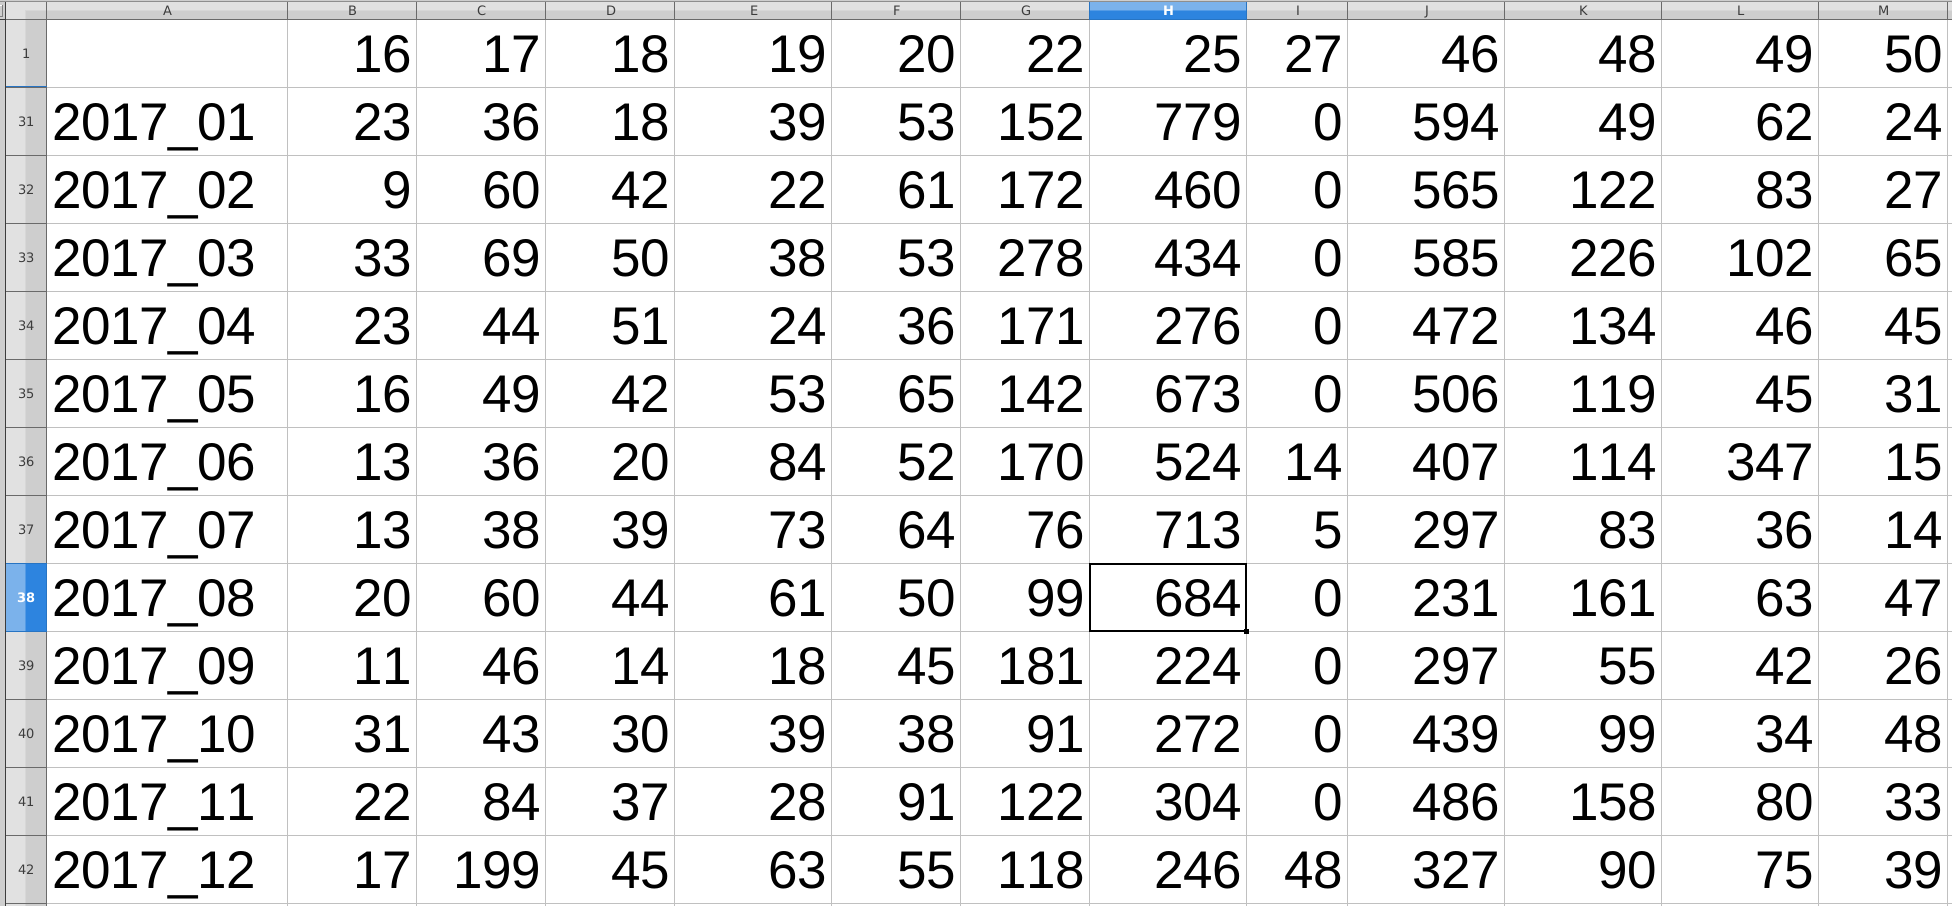
\includegraphics[height=\textheight]{downloadfigures.png}
}
\frame{
\frametitle{\mbox{Business data: Royalties}}
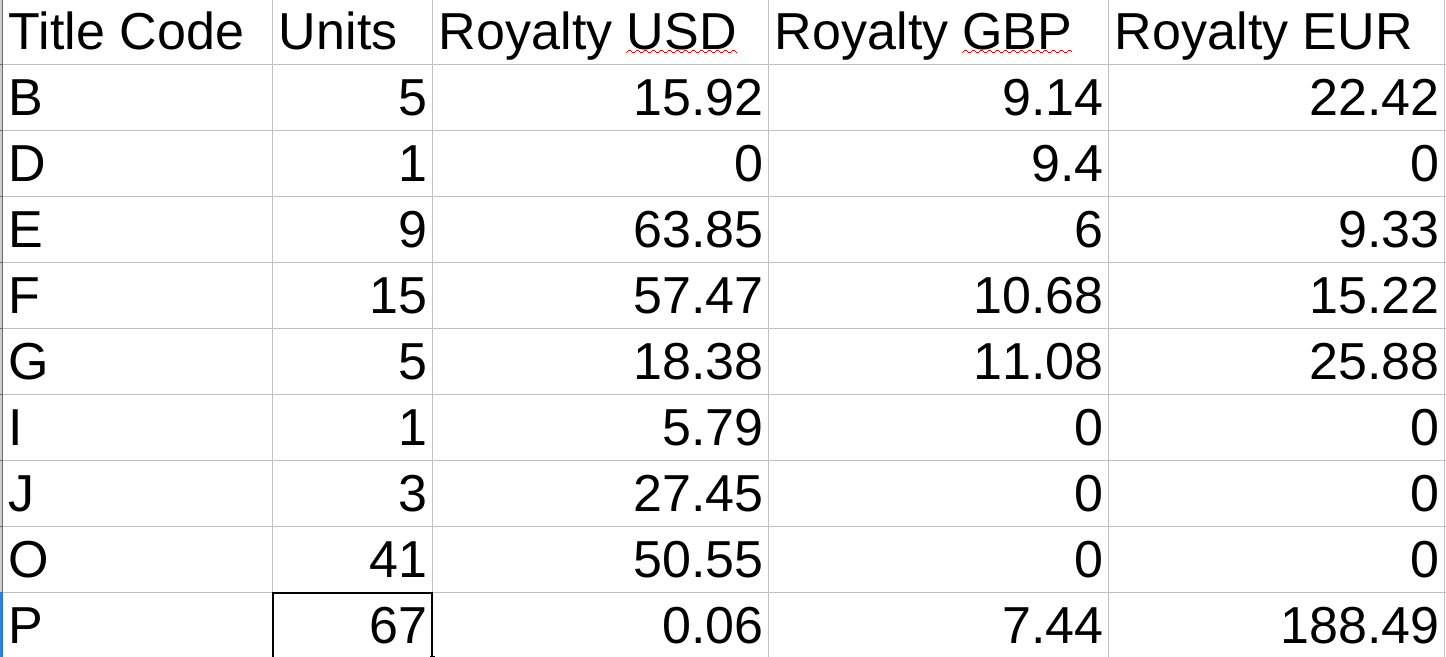
\includegraphics[width=\textwidth]{royalties.png}
}
\frame{
\frametitle{\mbox{Business data: BPCs}}
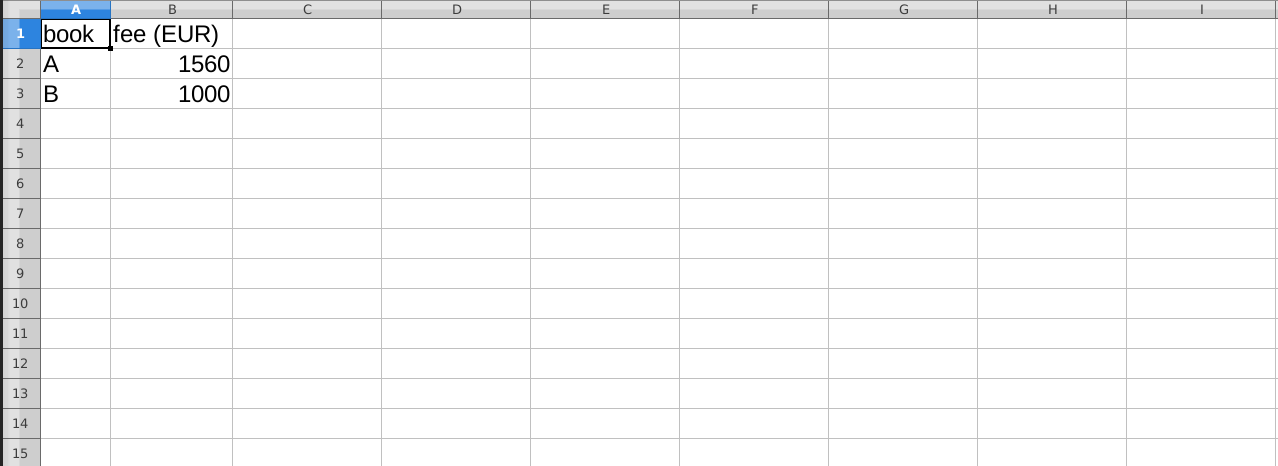
\includegraphics[height=\textheight]{apcs.png}
}


\section{Spreadsheet}
\frame{
\frametitle{Spreadsheet}
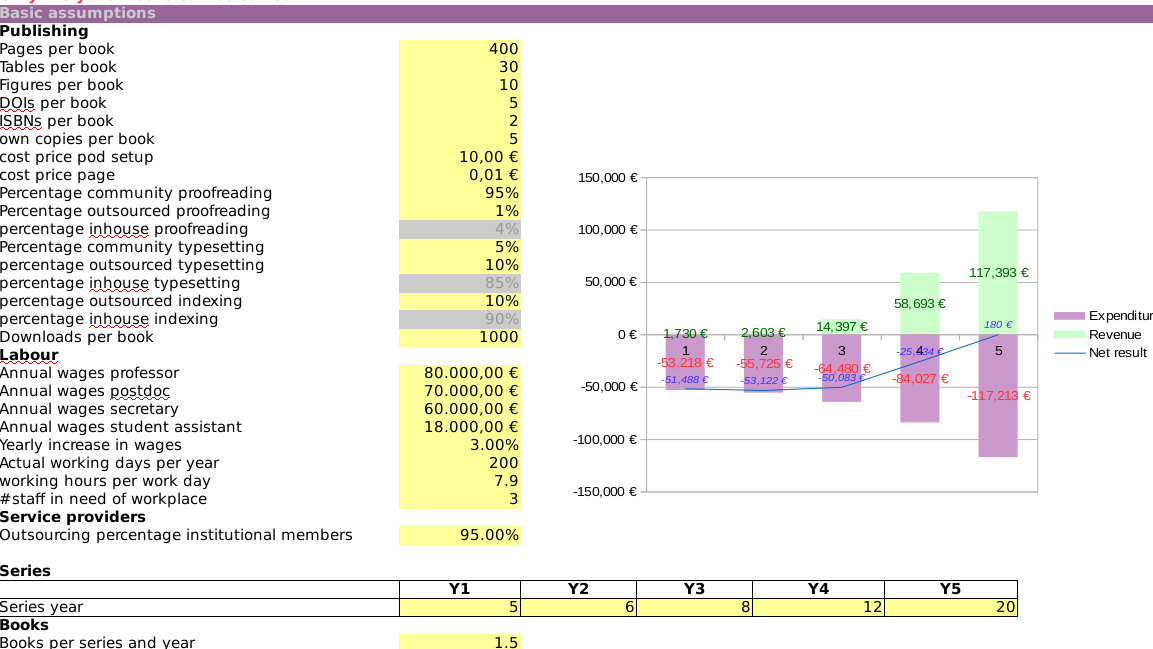
\includegraphics[height=\textheight]{5y.png}
}

\section{Business model}
\frame{
\frametitle{Business model}
\begin{columns}
  \begin{column}{6cm}
\begin{itemize}
 \item 70 page document
 \item original 2015 business model translated into English
 \item for each section: 
 \begin{itemize}
  \item background
  \item LangSci solution
  \item evaluation 
  \item alternative solutions
 \end{itemize}
 \item 5 revenue streams: BPCs, print margins, institutional members, individual members, donations
 \item take home message: go for consortial models!
\end{itemize}
  \end{column}
  \begin{column}{3cm}
    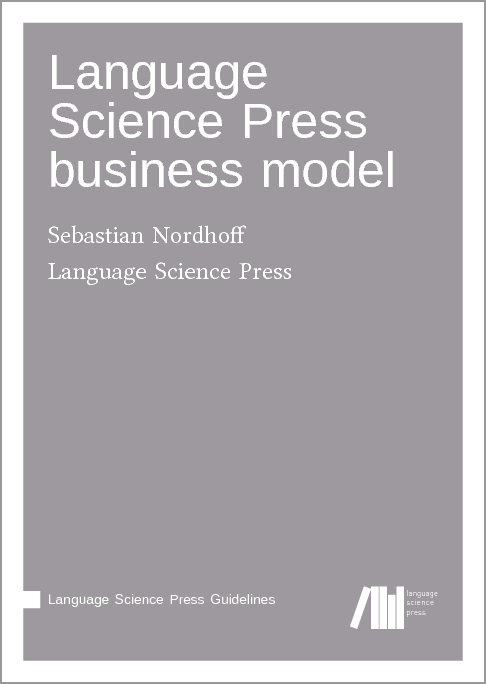
\includegraphics[width=3cm]{businessmodel}
  \end{column}
\end{columns}
}

\frame{
\frametitle{Why consortial models?}
\begin{tabular}{lrr}
Revenue stream & 
Projected& 
Realised\\
\hline	
Print margin&
24.000€ &5977€\\

Author fees
&48.000€
&2.500€
\\

Institutional memberships
&56.000€
&(85.000€)\\

Donations
&9.600€
&2.500€\\

Individual memberhships
&13.200€
&120€\\
\\
Context: books
&48
&26
\\
\hline
\end{tabular}

}


\section{Cookbook}
\frame{
\frametitle{Cookbook}
\begin{columns}
  \begin{column}{6cm}
\begin{itemize}
 \item 60 page document
 \item insights and lessons learned from the past 4 years
 \item prestige, community building, acquisition, workflow, print-on-demand, distribution, finance, legal 
\end{itemize}
  \end{column}
  \begin{column}{3cm}
    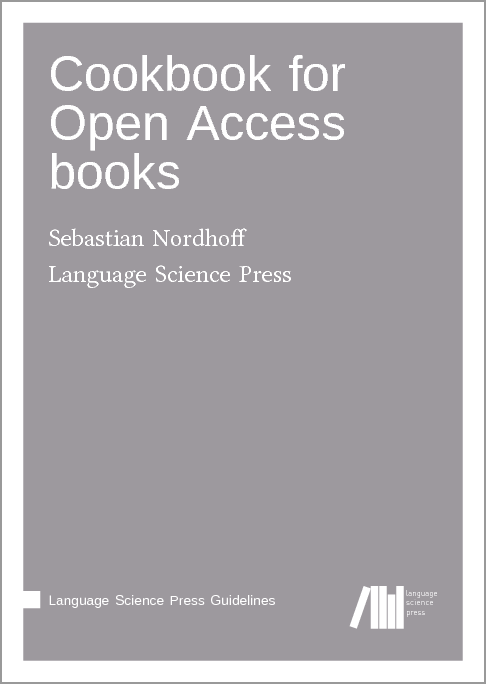
\includegraphics[width=3cm]{cookbook}
  \end{column}
\end{columns}
}


\frame{
\frametitle{Check it out}
\begin{tabular}{c|c}
 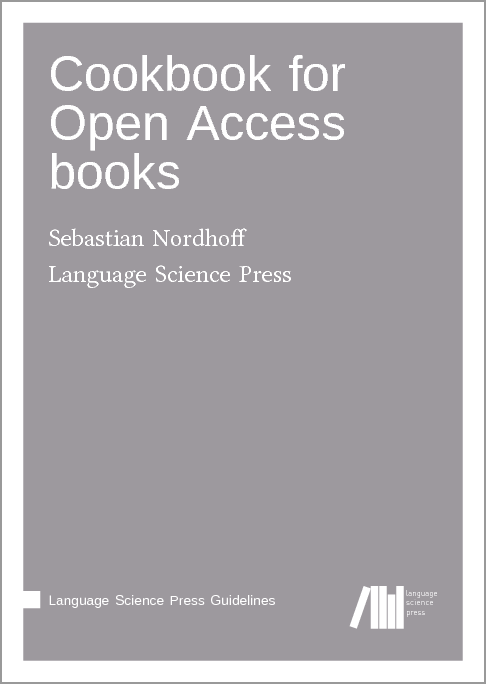
\includegraphics[height=3cm]{cookbook.png} &   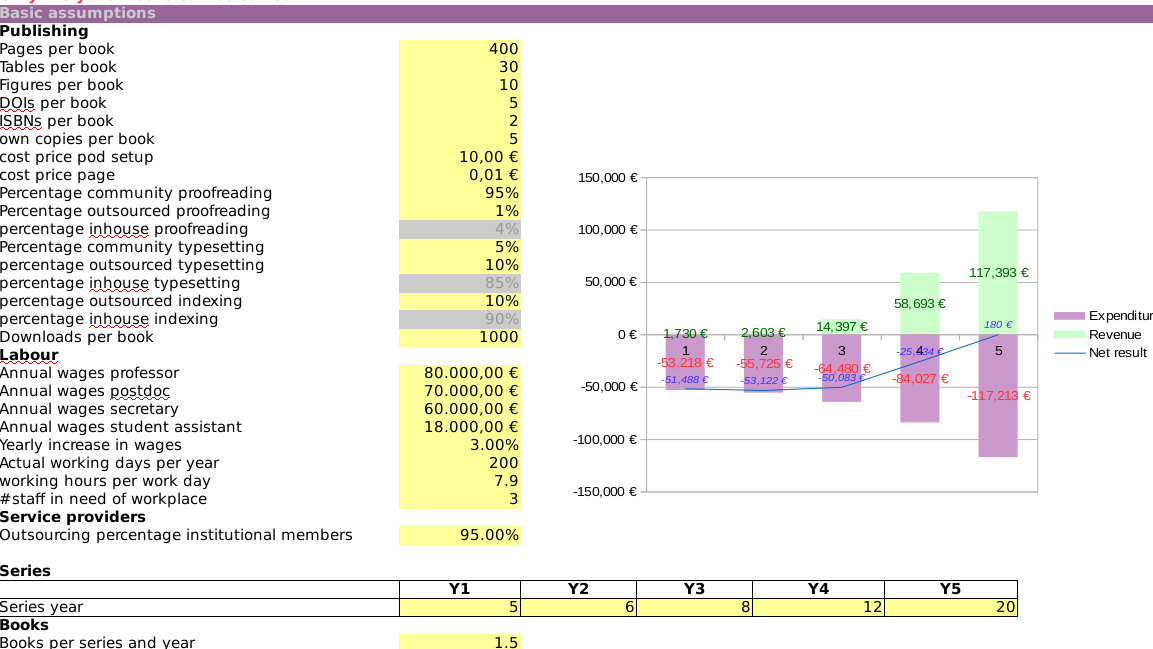
\includegraphics[height=2cm]{5y.png} \\  
 \hline\\
 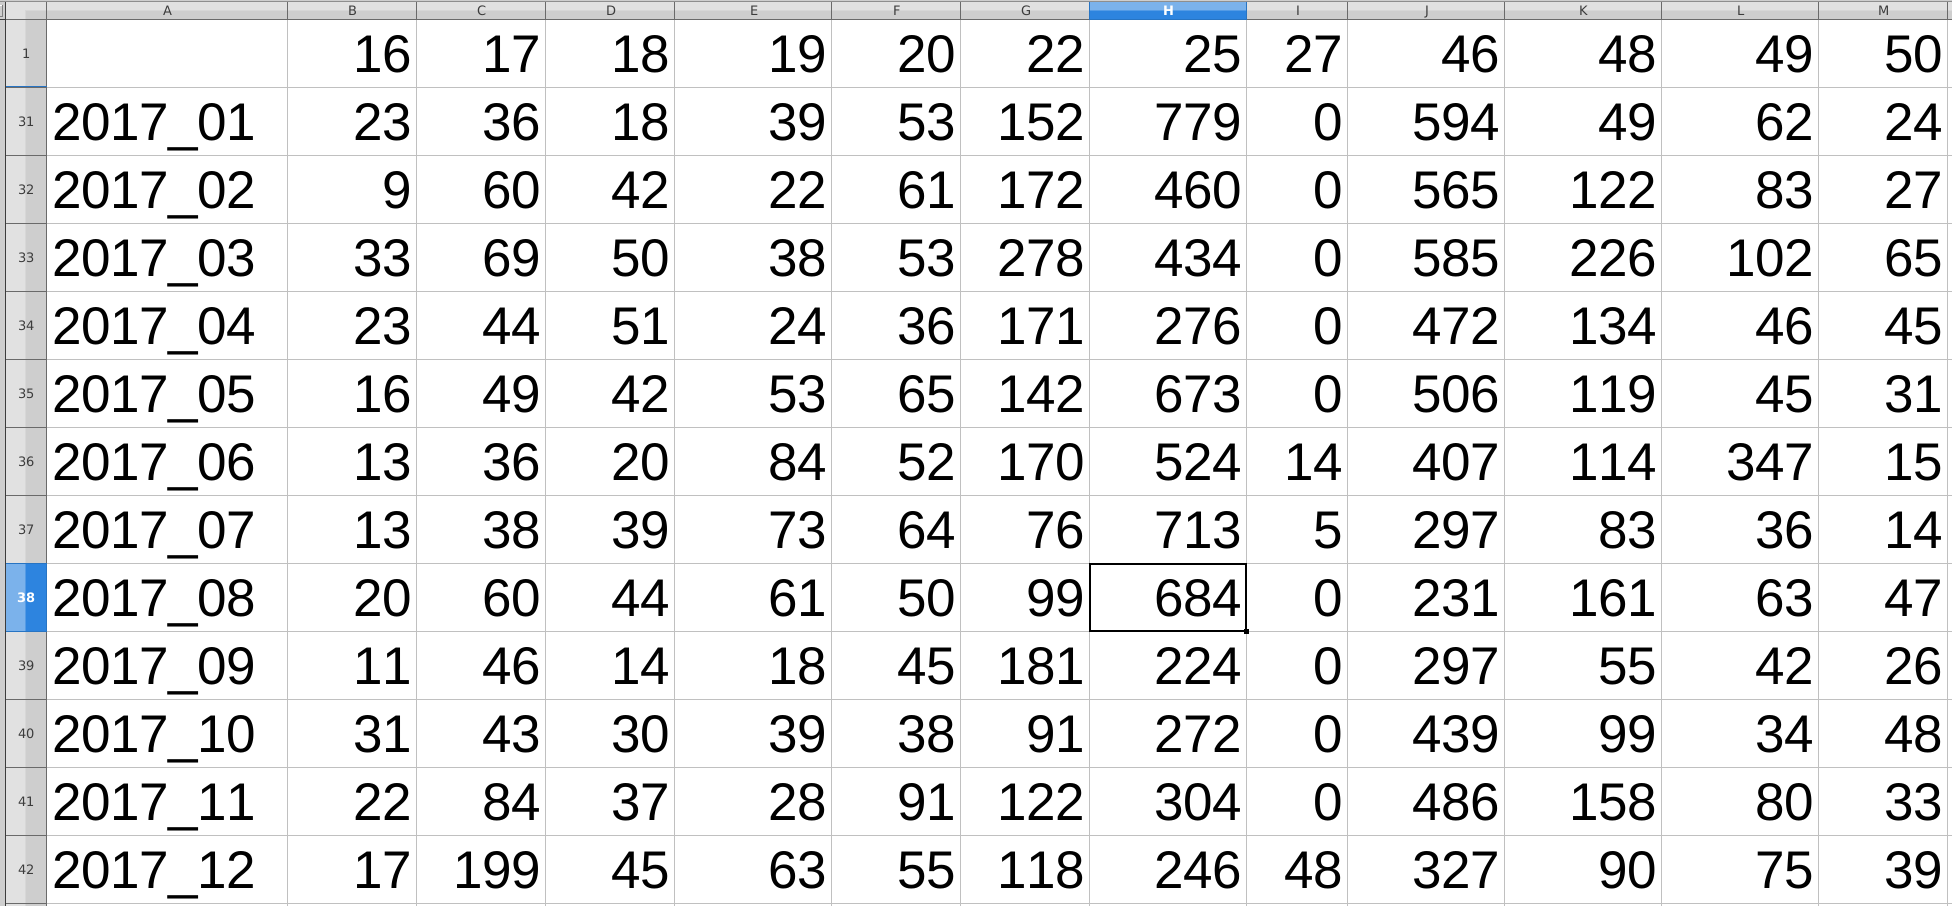
\includegraphics[height=2cm]{downloadfigures.png} &~\vspace*{13mm}~ 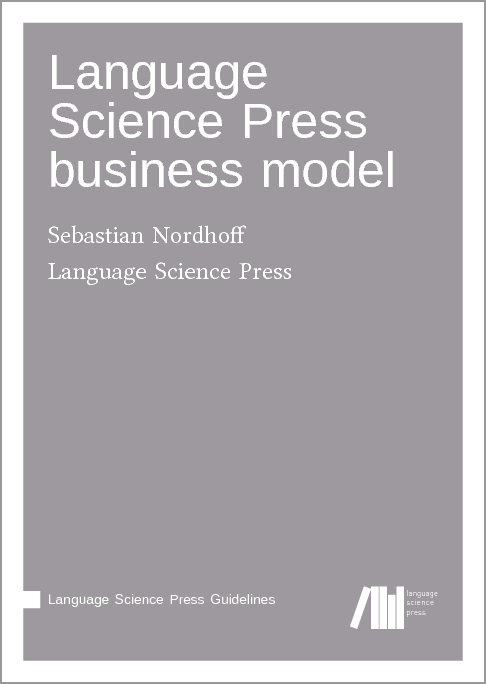
\includegraphics[height=3cm]{businessmodel.png} 
\end{tabular}
\vspace*{-1cm}
\begin{itemize}
 \item \url{github.com/langsci/opendata}, release on 2018-06-30
\end{itemize}


}

%\setcounter{framenumber}{\thelastpagemainpart}
\end{document}